\section*{Exercise 3}
\subsection*{a}

Let $d(x,y)$ be the distance from a point $P(x,y)$ to the center of the circle. Then the unit circle equation is $d(x,y) = 1$.

\begin{itemize}
    \item When $p = 1$, we have $x + y = 1$
    \item When $p = 2$, we have $\sqrt{x^2 + y^2} = 1$
    \item When $p = 10$, we have $(x^{10} + y^{10})^{\frac{1}{10}} = 1$
    \item When $p = \infty$, we have $max(x,y) = 1$
\end{itemize}

Plotting the graphs of those equations, we have the unit circles, shown in figure \ref{unit_circles}.

\begin{figure}[!htb]
  \centering
  \begin{subfigure}{0.49\textwidth}
    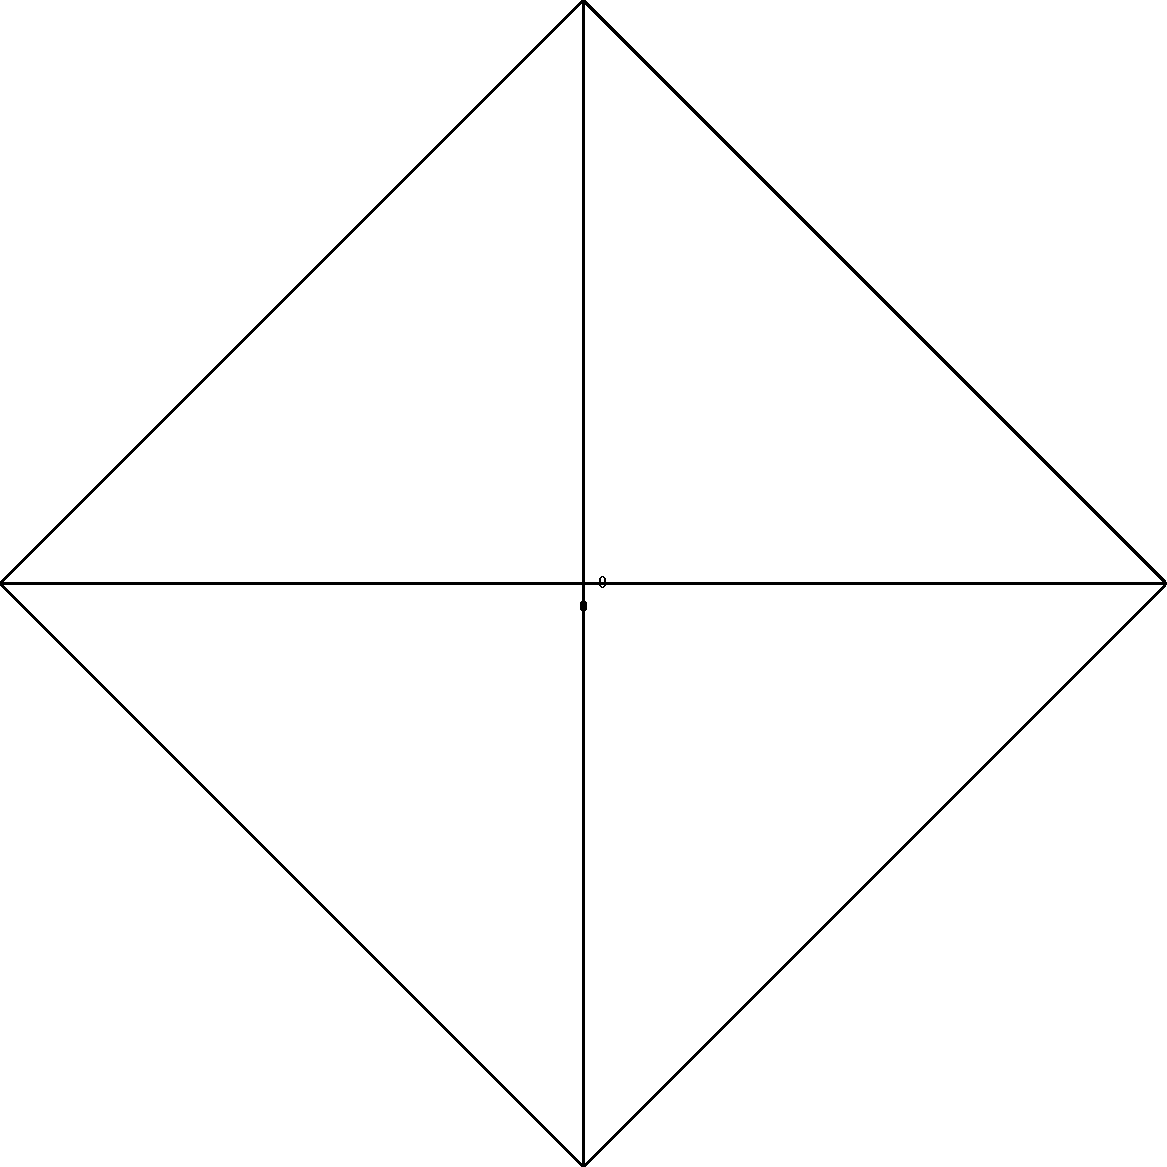
\includegraphics[width=0.5\textwidth]{shots/unit_circle_1}
    \caption{$p = 1$}
    \label{unit_circle_1}
  \end{subfigure}
  \begin{subfigure}{0.49\textwidth}
    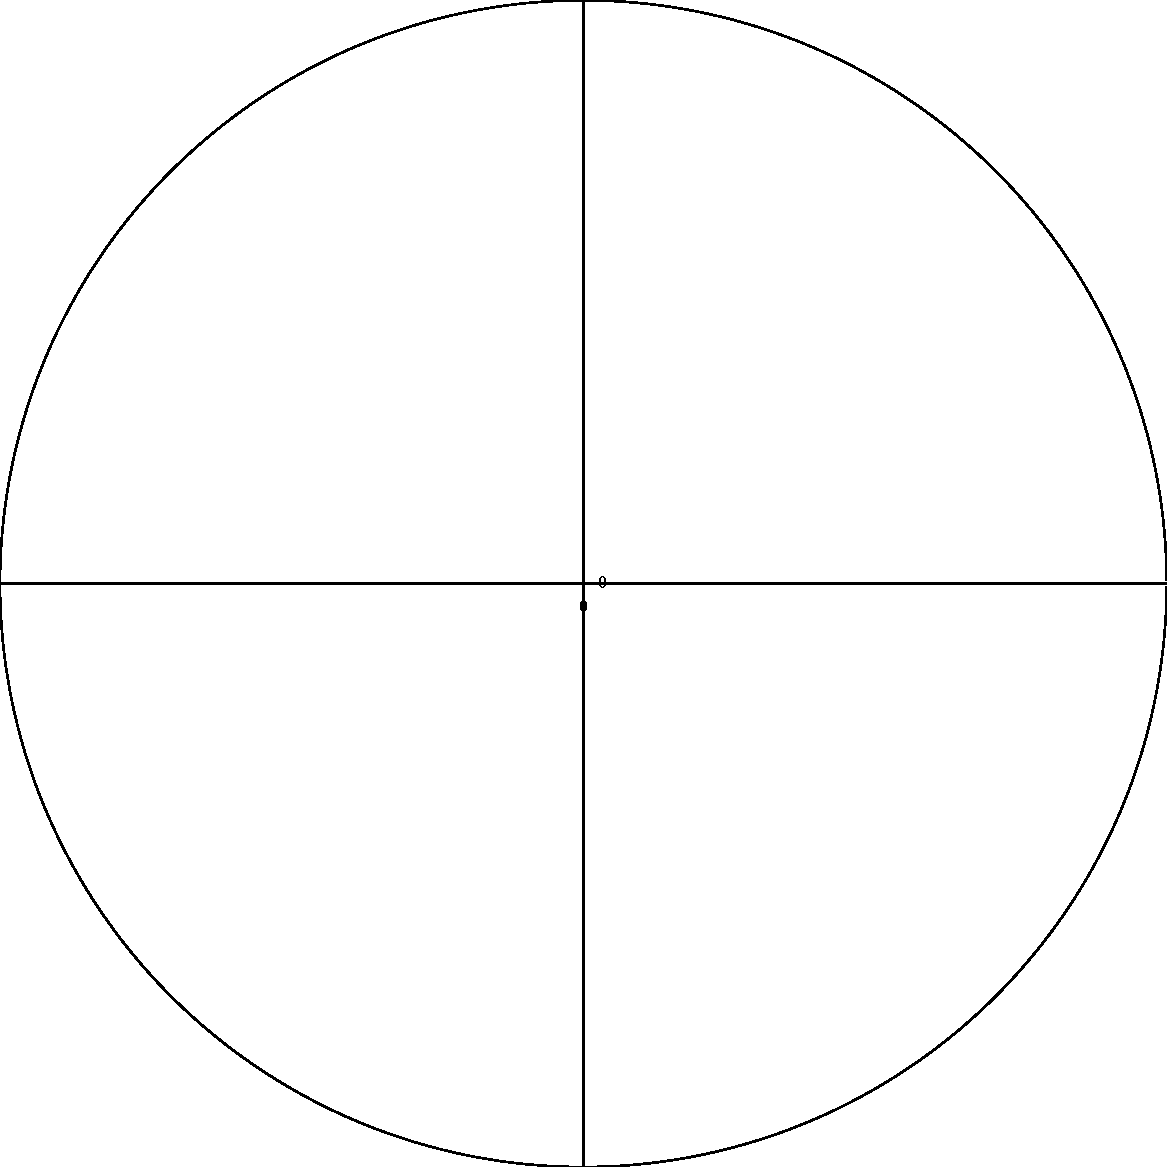
\includegraphics[width=0.5\textwidth]{shots/unit_circle_2}
    \caption{$p = 2$}
    \label{unit_circle_2}
  \end{subfigure}
  \begin{subfigure}{0.49\textwidth}
    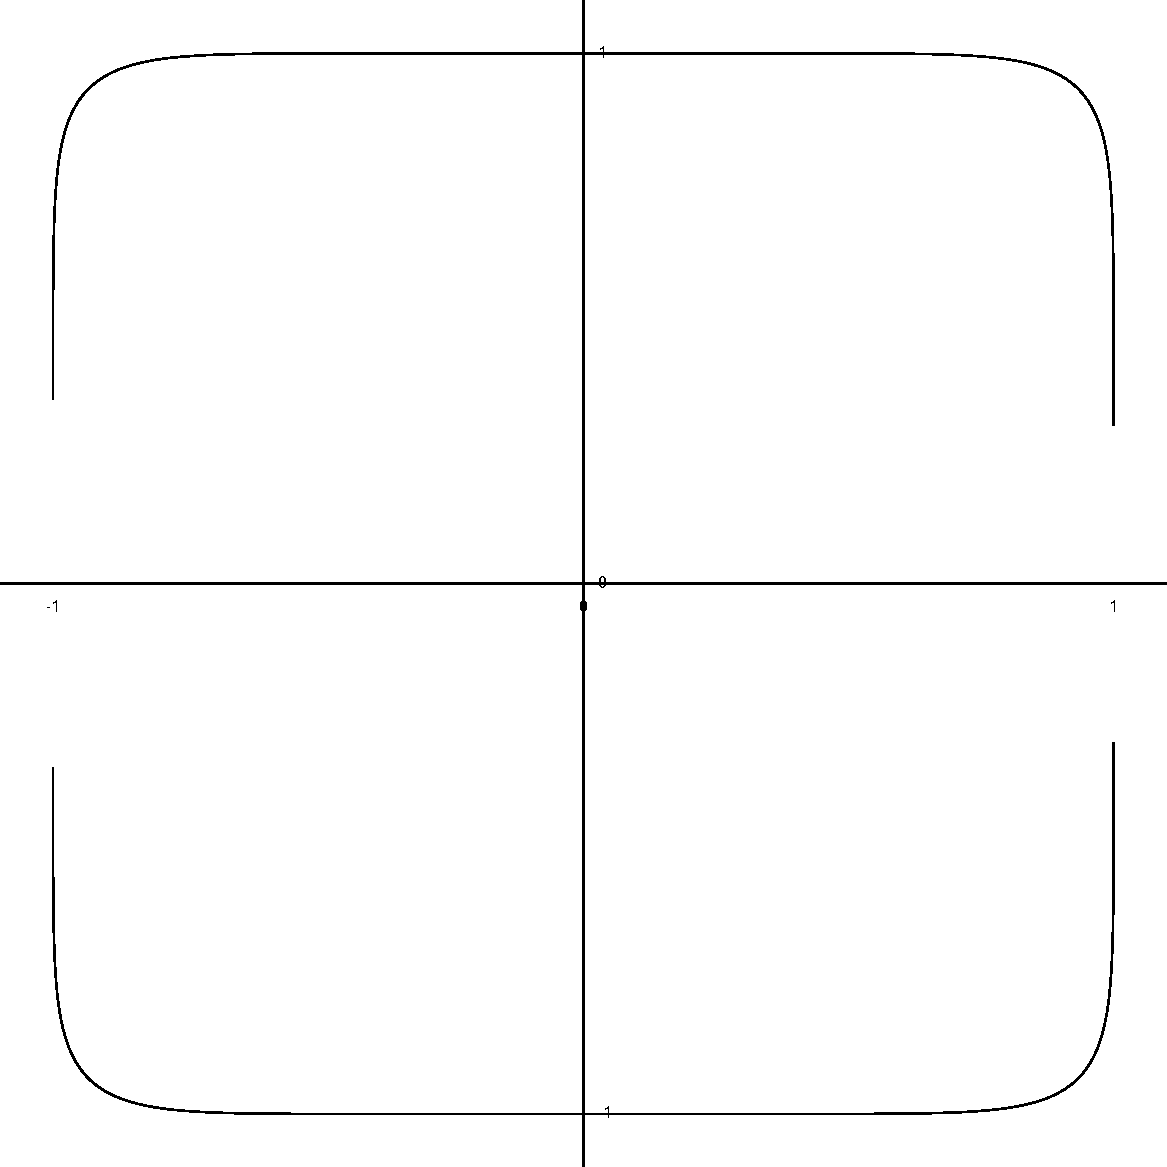
\includegraphics[width=0.5\textwidth]{shots/unit_circle_10}
    \caption{$p = 10$}
    \label{unit_circle_10}
  \end{subfigure}
  \begin{subfigure}{0.49\textwidth}
    
\includegraphics[width=0.5\textwidth]{shots/unit_circle_infi}
    \caption{$p = infi$}
    \label{unit_circle_infi}
  \end{subfigure}
  \caption{Unit Circles}
  \label{unit_circles}
\end{figure}

\subsection*{b}
We can see that the 2 unit circles (the 2 squares indeed) are quite similar. The differences are the angle ($pi/4$) and the length of the edge ($2$ and $\sqrt{2}$).
Thus, we can preserve the distance by doing a rotation by an angle of $pi/4$ followed by a scaling by a factor of$\sqrt{2}$.

The rotation matrix is:
$$
\begin{bmatrix}
  \sqrt{2}/2   & -\sqrt{2}/2  \\
  \sqrt{2}/2   & \sqrt{2}/2
\end{bmatrix}
$$

So the mapping function can be done by multiplying the following matrix to the original data:

$$
\begin{bmatrix}
  1 & -1  \\
  1 & 1 
\end{bmatrix}
$$

Now we prove that the mapping function actually preserves the distance. As we know, the difference between 2 vectors is also a vector. Let $p = (a, b)$ be a difference
between 2 vectors in space. After the transformation, $p' = (a - b, a + b)$. We have:

\begin{align*}
  ||p||_1 &= |a| + |b| \\
  ||p'||_\infty &= max(|a - b|, |a + b|) = |a| + |b|
\end{align*}

So $||p||_1 = ||p'||_\infty$. This completes the proof.
